\chapter{The Epsilon Wizard Language (EWL)}
\label{sec:EWL}

There are two types of model-to-model transformations: mapping and update transformations \cite{Czarnecki2003}. Mapping transformations typically transform a source model into a set of target models expressed in (potentially) different modelling languages by creating zero or more model elements in the target models for each model element of the source model. By contrast, update transformations perform in-place modifications in the source model itself. They can be further classified into two subcategories: transformations in the small and in the large. Update transformations in the large apply to sets of model elements calculated using well-defined rules in a batch manner. An example of this category of transformations is a transformation that automatically adds accessor and mutator operations for all attributes in a UML model. On the other hand, update transformations in the small are applied in a user-driven manner on model elements that have been explicitly selected by the user. An example of this kind of transformations is a transformation that renames a \emph{user-specified} UML class and all its incoming associations consistently.

In Epsilon, mapping transformations can be specified using ETL as discussed in Section \ref{sec:ETL}, and update transformations in the large can be implemented either using the model modification features of EOL or using an ETL transformation in which the source and target models are the same model. By contrast, update transformations in the small cannot be effectively addressed by any of the languages presented so far.

The following section discusses the importance of update transformations in the small and motivates the definition of a task-specific language (Epsilon Wizard Language (EWL)) that provides tailored and effective support for defining and executing update transformations on models of diverse metamodels.

\section{Motivation}
\label{sec:EwlMotivation}

Constructing and refactoring models is undoubtedly a mentally intensive process. However, during modelling, recurring patterns of model update activities typically appear. As an example, when renaming a class in a UML class diagram, the user also needs to manually update the names of association ends that link to the renamed class. Thus, when renaming a class from \emph{Chapter} to \emph{Section}, all associations ends that point to the class and are named \emph{chapter} or \emph{chapters} should be also renamed to \emph{section} and \emph{sections} respectively. As another example, when a modeller needs to refactor a UML class into a singleton \cite{Larman}, they need to go through a number of well-defined, but trivial, steps such as attaching a stereotype ($<<singleton>>$), defining a static \emph{instance} attribute and adding a static \emph{getInstance()} method that returns the unique instance of the singleton.

It is generally accepted that performing repetitive tasks manually is both counter-productive and error-prone \cite{CG.InAction}. On the other hand, failing to complete such tasks correctly and precisely compromises the consistency, and thus the quality, of the models. In Model Driven Engineering, this is particularly important since models are increasingly used to automatically produce (parts of) working systems. 

\subsection{Automating the Construction and Refactoring Process}

Contemporary modelling tools provide built-in transformations (\textit{wizards}) for automating common repetitive tasks. However, according to the architecture of the designed system and the specific problem domain, additional repetitive tasks typically appear, which cannot be addressed by the pre-conceived built-in wizards of a modelling tool. To address the automation problem in its general case, users must be able to easily define update transformations (wizards) that are tailored to their specific needs.

To an extent, this can be achieved via the extensible architecture that state-of-the-art modelling tools often provide which enables users to add functionality to the tool via scripts or application code using the implementation language of the tool. Nevertheless, as discussed in \cite{EOL}, the majority of modelling tools provide an API through which they expose an edited model, which requires significant effort to learn and use. Also, since each API is proprietary, such scripts and extensions are not portable to other tools. Finally, API scripting languages and third-generation languages such as Java and C++ are not particularly suitable for model navigation and modification \cite{EOL}.

Furthermore, existing languages for mapping transformations, such as QVT, ATL and ETL, cannot be used as-is for this purpose, because these languages have been designed to operate in a batch manner without human involvement in the process. By contrast, as discussed above, the task of constructing and refactoring models is inherently user-driven.

\section{Update Transformations in the Small}
\label{sec:ModelTransformationInTheSmall}

Update transformations are actions that automatically create, update or delete model elements based on a selection of existing elements in the model and information obtained otherwise (e.g. through user input), in a user-driven fashion. In this section, such actions are referred to as \textit{wizards} instead of \textit{rules} to reduce confusion between them and rules of mapping transformation languages. In the following sections, the desirable characteristics of wizards are elaborated informally. 

\subsection{Structure of Wizards}

In its simplest form, a wizard only needs to define the actions it will perform when it is applied to a selection of model elements. The structure of such a wizard that transforms a UML class into a \textit{singleton} is shown using pseudo-code in Listing \ref{lst:Basic}.\\

\begin{lstlisting}[caption=The simplest form of a wizard for refactoring a class into a singleton, label=lst:Basic, language=EWL]
do :
	attach the singleton stereotype
	create the instance attribute
	create the getInstance method
\end{lstlisting}

Since not all wizards apply to all types of elements in the model, each wizard needs to specify the types of elements to which it applies. For example, the wizard of Listing \ref{lst:Basic}, which automatically transforms a class into a singleton, applies only when the selected model element is a class. The simplest approach to ensuring that the wizard will only be applied on classes is to enclose its body in an \emph{if} condition as shown in Listing \ref{lst:WithoutGuard}.

\begin{lstlisting}[caption=The wizard of Listing \ref{lst:Basic} enhanced with an $if$ condition, label=lst:WithoutGuard, language=EWL]
do : 
	if (selected element is a class) {
		attach the singleton stereotype
		create the instance attribute
		create the getInstance method
	}
\end{lstlisting}

A more modular approach is to separate this condition from the body of the wizard. This is shown in Listing \ref{lst:WithGuard} where the condition of the wizard is specified as a separate \emph{guard} stating that the wizard applies only to elements of type Class. The latter is preferable since it enables filtering out wizards that are not applicable to the current selection of elements by evaluating only their \emph{guard} parts and rejecting those that return \emph{false}. Thus, at any time, the user can be provided with only the wizards that are applicable to the current selection of elements. Filtering out irrelevant wizards reduces confusion and enhances usability, particularly as the list of specified wizards grows.

\begin{lstlisting}[caption=The wizard of Listing \ref{lst:WithoutGuard} with an explicit $guard$ instead of the $if$ condition, label=lst:WithGuard, language=EWL]
guard : selected element is a class
do : 
	attach the singleton stereotype
	create the instance attribute
	create the getInstance method
\end{lstlisting}

To enhance usability, a wizard also needs to define a short human-readable description of its functionality. To achieve this, another field named \emph{title} has been added. There are two options for defining the title of a wizard: the first is to use a static string and the second to use a dynamic expression. The latter is preferable since it enables definition of context-aware titles.

\begin{lstlisting}[caption=The wizard of Listing \ref{lst:WithGuard} enhanced with a $title$ part, label=lst:FinalForm, language=EWL]
guard : selected element is a class
title : Convert class <class-name> into a singleton
do : 
	attach the singleton stereotype
	create the instance attribute
	create the getInstance method
\end{lstlisting}

\subsection{Capabilities of Wizards}

The \emph{guard} and \emph{title} parts of a wizard need to be expressed using a language that provides model querying and navigation facilities. Moreover, the \emph{do} part also requires model modification capabilities to implement the transformation. To achieve complex transformations, it is essential that the user can provide additional information. For instance, to implement a wizard that addresses the class renaming scenario discussed in Section \ref{sec:EwlMotivation}, the information provided by the selected class does not suffice; the user must also provide the new name of the class. Therefore, EWL must also provide mechanisms for capturing user input.

\section{Abstract Syntax}

Since EWL is built atop Epsilon, its abstract and concrete syntax need only to define the concepts that are relevant to the task it addresses; they can reuse lower-level constructs from EOL. A graphical overview of the abstract syntax of the language is provided in Figure \ref{fig:EwlAbstractSyntax}. 

The basic concept of the EWL abstract syntax is a \emph{Wizard}. A wizard defines a \emph{name}, a \emph{guard} part, a \emph{title} part and a $do$ part. Wizards are organized in \emph{Modules}. The \emph{name} of a wizard acts as an identifier and must be unique in the context of a module. The \emph{guard} and \emph{title} parts of a wizard are of type \emph{ExpressionOrStatementBlock}, inherited from EOL. An \emph{ExpressionOrStatementBlock} is either a single EOL expression or a block of EOL statements that include one or more \emph{return} statements. This construct allows users to express simple declarative calculations as single expressions and complex calculations as blocks of imperative statements. The usefulness of this construct is further discussed in the examples presented in Section \ref{sec:EwlExamples}. Finally, the \emph{do} part of the wizard is a block of EOL statements that specify the effects of the wizard when applied to a compatible selection of model elements. 

\begin{figure}
	\centering
		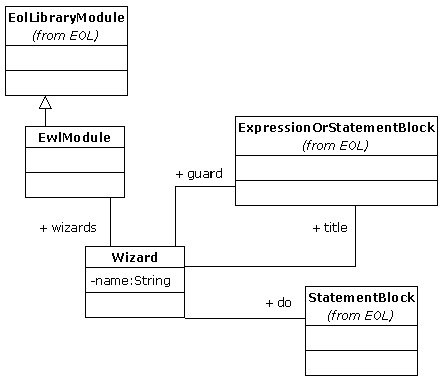
\includegraphics{images/EwlAbstractSyntax.png}
	\caption{EWL Abstract Syntax}
	\label{fig:EwlAbstractSyntax}
\end{figure}

\clearpage

\section{Concrete Syntax}

Listing \ref{lst:EwlConcreteSyntax} presents the concrete syntax of EWL wizards.

\begin{lstlisting}[caption=Concrete syntax of EWL wizards, label=lst:EwlConcreteSyntax, language=EWL, escapechar=!]
wizard !\textit{<name>}! {
	(guard (!\textbf{:}\textit{expression}!)|(!\textbf{\{}\textit{statementBlock}\textbf{\}}!))?
	(title (!\textbf{:}\textit{expression}!)|(!\textbf{\{}\textit{statementBlock}\textbf{\}}!))?
	do {
		statementBlock
	}
}
\end{lstlisting}

\section{Execution Semantics}
The process of executing EWL wizards is inherently user-driven and as such it depends on the environment in which they are used. In general, each time the selection of model elements changes (i.e. the user selects or deselects a model element in the modelling tool), the guards of all wizards are evaluated. If the guard of a wizard is satisfied, the \emph{title} part is also evaluated and the wizard is added to a list of \textit{applicable} wizards. Then, the user can select a wizard and execute its \emph{do} part to perform the intended transformation.

In EWL, variables defined and initialized in the \emph{guard} part of the wizard can be accessed both by the \emph{title} and the \emph{do} parts. In this way, results of calculations performed in the \emph{guard} part can be re-used, instead of re-calculated in the subsequent parts.  The practicality of this approach is discussed in more detail in the examples that follow. Also, the execution of the \emph{do} part of each wizard is performed in a transactional mode by exploiting the transaction capabilities of the underlying model connectivity framework, so that possible logical errors in the \emph{do} part of a wizard do not leave the edited model in an inconsistent state. 

\section{Examples}
\label{sec:EwlExamples}

This section presents three concrete examples of EWL wizards for refactoring UML 1.4 models. The aim of this section is not to provide complete implementations that address all the sub-cases of each scenario but to provide enhanced understanding of the concrete syntax, the features and the capabilities of EWL to the reader. Moreover, it should be stressed again that although the examples in this section are based on UML models, by building on Epsilon, EWL can be used to capture wizards for diverse modelling languages and technologies.

\subsubsection{Converting a Class into a Singleton}
\label{sec:ClassToSingleton}

The singleton pattern \cite{Larman} is applied when there is a class for which only one instance can exist at a time. In terms of UML, a singleton is a class stereotyped with the $<<singleton>>$ stereotype, and it defines a static attribute named \emph{instance} which holds the value of the unique instance. It also defines a static \emph{getInstance()} operation that returns that unique instance. Wizard \emph{ClassToSingleton}, presented in Listing \ref{lst:ClassToSingleton}, simplifies the process of converting a class into a singleton by adding the proper stereotype, attribute and operation to it automatically.

\begin{lstlisting}[ 
	basicstyle=\ttfamily\footnotesize, 
	flexiblecolumns=true,
	numbers=none,
	nolol=true,
	caption=Implementation of the ClassToSingleton Wizard, 
	label=lst:ClassToSingleton,
	numbers=left,
	language=EWL,
	tabsize=2
]
wizard ClassToSingleton {
	
	// The wizard applies when a class is selected
	guard : self.isTypeOf(Class)
	
	title : "Convert " + self.name + " to a singleton"
	
	do {
		// Create the getInstance() operation 
		var gi : new Operation; 
		gi.owner = self; 
		gi.name = "getInstance"; 
		gi.visibility = VisibilityKind#vk_public; 
		gi.ownerScope = ScopeKind#sk_classifier; 
		
		// Create the return parameter of the operation 
		var ret : new Parameter; 
		ret.type = self; 
		ret.kind = ParameterDirectionKind#pdk_return; 
		gi.parameter = Sequence{ret}; 
		
		// Create the instance field 
		var ins : new Attribute; 
		ins.name = "instance"; 
		ins.type = self; 
		ins.visibility = VisibilityKind#vk_private; 
		ins.ownerScope = ScopeKind#sk_classifier; 
		ins.owner = self; 
		
		// Attach the <<singleton>> stereotype 
		self.attachStereotype("singleton");
	}
}

// Attaches a stereotype with the specified name
// to the Model Element on which it is invoked
operation ModelElement attachStereotype(name : String) {
		var stereotype : Stereotype;
		
		// Try to find an existing stereotype with this name
		stereotype = Stereotype.allInstances.selectOne(s|s.name = name);
		
		// If there is no existing stereotype
		// with that name, create one
		if (not stereotype.isDefined()){
			stereotype = Stereotype.createInstance();
			stereotype.name = name;
			stereotype.namespace = self.namespace;
		}
		
		// Attach the stereotype to the model element
		self.stereotype.add(stereotype);
}
\end{lstlisting}

The \emph{guard} part of the wizard specifies that it is only applicable when the selection is a single UML class. The \emph{title} part specifies a context-aware title that informs the user of the functionality of the wizard and the \emph{do} part implements the functionality by adding the \emph{getInstance} operation (lines 10-14), the \emph{instance} attribute (lines 23-28) and the $<<singleton>>$ stereotype (line 31). 

The stereotype is added via a call to the \emph{attachStereotype()} operation. Attaching a stereotype is a very common action when refactoring UML models, particularly where UML profiles are involved, and therefore to avoid duplication, this reusable operation that checks for an existing stereotype, creates it if it does not already exists, and attaches it to the model element on which it is invoked has been specified.

An extended version of this wizard could also check for existing association ends that link to the class and for which the upper-bound of their multiplicity is greater than one and either disallow the wizard from executing on such classes (in the $guard$ part) or update the upper-bound of their multiplicities to one (in the $do$ part). However, the aim of this section is not to implement complete wizards that address all sub-cases but to provide a better  understanding of the concrete syntax and the features of EWL. This principle also applies to the examples presented in the sequel.
\subsubsection{Renaming a Class}
\label{sec:RenameClass}

The most widely used convention for naming attributes and association ends of a given class is to use a lower-case version of the name of the class as the name of the attribute or the association end. For instance, the two ends of a one-to-many association that links classes \texttt{Book} and \texttt{Chapter} are most likely to be named \texttt{book} and \texttt{chapters} respectively. When renaming a class (e.g. from \texttt{Chapter} to \texttt{Section}) the user must then manually traverse the model to find all attributes and association ends of this type and update their names (i.e. from \texttt{chapter} or \texttt{bookChapter} to \texttt{section} and \texttt{bookSection} respectively). This can be a daunting process especially in the context of large models. Wizard \texttt{RenameClass} presented in Listing \ref{lst:RenameClass} automates this process.

\begin{lstlisting}[ 
	basicstyle=\ttfamily\footnotesize, 
	flexiblecolumns=true, 
	numbers=none, 
	nolol=true, 
	caption=Implementation of the RenameClass Wizard,
	label=lst:RenameClass, 
	numbers=left, 
	language=EWL, 
	tabsize=2
]
wizard RenameClass {
	
	// The wizard applies when a Class is selected
	guard : self.isKindOf(Class)
	
	title : "Rename class " + self.name
	
	do {
		var newName : String;
		
		// Prompt the user for the new name of the class
		newName = UserInput.prompt("New name for class " + self.name);
		if (newName.isDefined()) {
			var affectedElements : Sequence;
			
			// Collect the AssociationEnds and Attributes
			// that are affected by the rename
			affectedElements.addAll(
				AssociationEnd.allInstances.select(ae|ae.participant=self));
			affectedElements.addAll(
				Attribute.allInstances.select(a|a.type = self));
			
			var oldNameToLower : String;
			oldNameToLower = self.name.firstToLowerCase();
			var newNameToLower : String;
			newNameToLower = newName.firstToLowerCase();
			
			// Update the names of the affected AssociationEnds
			// and Attributes
			for (ae in affectedElements) {
					ae.replaceInName(oldNameToLower, newNameToLower);
					ae.replaceInName(self.name, newName);
			}
			self.name = newName;
		}
	}
	
}

// Renames the ModelElement on which it is invoked
operation ModelElement replaceInName
	(oldString : String, newString : String) {
	
	if (oldString.isSubstringOf(self.name)) {
		// Calculate the new name
		var newName : String;
		newName = self.name.replace(oldString, newString);
		
		// Prompt the user for confirmation of the rename
		if (UserInput.confirm
			("Rename " + self.name + " to " + newName + "?")) {
			// Perform the rename
			self.name = newName;
		}
	}
}
\end{lstlisting}
%\vspace{-8pt}
As with the \texttt{ClassToSingleton} wizard, the \texttt{guard} part of \texttt{RenameClass} specifies that the wizard is applicable only when the selection is a simple class and the \emph{title} provides a context-aware description of the functionality of the wizard. 

As discussed in Section \ref{sec:ModelTransformationInTheSmall}, the information provided by the selected class itself does not suffice in the case of renaming since the new name of the class is not specified anywhere in the existing model. In EWL, and in all languages that build on EOL, user input can be obtained using the built-in \texttt{UserInput} facility. Thus, in line 12 the user is prompted for the new name of the class using the \texttt{UserInput.prompt()} operation. Then, all the association ends and attributes that refer to the class are collected in the \texttt{affectedElements} sequence (lines 14-21). Using the \texttt{replaceInName} operation (lines 31 and 32), the name of each one is examined for a substring of the upper-case or the lower-case version of the old name of the class. In case the check returns true, the user is prompted to confirm (line 48) that the feature needs to be renamed. This further highlights the importance of user input for implementing update transformations with fine-grained user control. 
\subsubsection{Moving Model Elements into a Different Package}
\label{sec:MoveToPackage}

A common refactoring when modelling in UML is to move model elements, particularly Classes, between different packages. When moving a pair of classes from one package to another, the associations that connect them must also be moved to the target package. To automate this process, Listing \ref{lst:MoveToPackage} presents the \texttt{MoveToPackage} wizard.

\begin{lstlisting}[
	basicstyle=\ttfamily\footnotesize, 
	flexiblecolumns=true, 
	numbers=none, 
	nolol=true, 
	caption=Implementation of the MoveToPackage Wizard, 
	label=lst:MoveToPackage, 
	numbers=left, 
	language=EWL, 
	tabsize=2
]
wizard MoveToPackage {
	
	// The wizard applies when a Collection of
	// elements, including at least one Package
	// is selected
	guard { 
		var moveTo : Package;
		if (self.isKindOf(Collection)) {
			moveTo = self.select(e|e.isKindOf(Package)).last();
		}
		return moveTo.isDefined();
	}
	
	title : "Move " + (self.size()-1) + " elements to " + moveTo.name
	
	do {
		// Move the selected Model Elements to the
		// target package
		for (me in self.excluding(moveTo)) {
			me.namespace = moveTo;
		}
		
		// Move the Associations connecting any
		// selected Classes to the target package
		for (a in Association.allInstances) {
			if (a.connection.forAll(c|self.includes(c.participant))){
				a.namespace = moveTo;
			}
		}
	}
	
}
\end{lstlisting}

The wizard applies when more than one element is selected and at least one of the elements is a \emph{Package}. If more than one package is selected, the last one is considered as the target package to which the rest of the selected elements will be moved. This is specified in the \emph{guard} part of the wizard.

To reduce user confusion in identifying the package to which the elements will be moved, the name of the target package appears in the title of the wizard. This example shows the importance of the decision to express the title as a dynamically calculated expression (as opposed to a static string). It is worth noting that in the \emph{title} part of the wizard (line 14), the \emph{moveTo} variable declared in the \emph{guard} (line 7) is referenced. Through experimenting with a number of wizards, it has been noticed that in complex wizards repeated calculations need to be performed in the \emph{guard}, \emph{title} and \emph{do} parts of the wizard. To eliminate this duplication, the scope of variables defined in the \emph{guard} part has been extended so that they are also accessible from the \emph{title} and \emph{do} part of the wizard.


\section{Summary}

This section has presented the Epsilon Wizard Language (EWL), a language for specifying and executing update transformations in the small on models of diverse metamodels. EWL provides a textual concrete syntax tailored to the task and features such as dynamically calculated wizard titles, transactional execution of the \emph{do} parts of wizards and user interaction.